\chapter{Structured P2P and the Transport Layer}
\section{Structured P2P Systems}
\begin{itemize}[nosep]
    \item Distributed Hash Table (DHT)
          \begin{itemize}[nosep]
              \item Efficient $(\texttt{Key}, \texttt{Value})$ storage
              \item Approach: map the ID to a host
          \end{itemize}
    \item Challenges
          \begin{itemize}[nosep]
              \item Scale to millions of nodes
              \item Churn
              \item Heterogeneity
          \end{itemize}
\end{itemize}
\subsection{DHTs}
\begin{itemize}[nosep]
    \item IDs from a \emph{flat} namespace
          \begin{itemize}[nosep]
              \item Contrast with hierarchical IP, DNS
          \end{itemize}
    \item Metaphor: hash table, but distributed
    \item Interface
          \begin{itemize}[nosep]
              \item $\textproc{Get}(\texttt{key})$
              \item $\textproc{Put}(\texttt{key}, \texttt{value})$
          \end{itemize}
    \item How?
          \begin{itemize}[nosep]
              \item Every node supports a single operation:

                    Given a \texttt{key}, route messages to node holding \texttt{key}
          \end{itemize}
\end{itemize}
\subsubsection{Consistent Hashing}
\begin{itemize}[nosep]
    \item Map keys to nodes
    \item $\texttt{nodeID} = \textproc{hash}(\texttt{nodeIP})$
    \item $k$ mapped to $\textproc{successor}(k)$
    \item $\textproc{successor}(k)$ is the first active node beginning at $k$
\end{itemize}
\begin{figure}[H]
    \tikzsetnextfilename{consistent-hashing}
    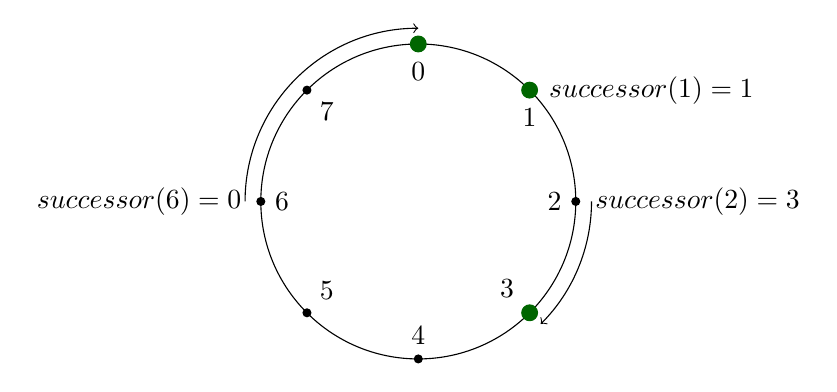
\begin{tikzpicture}[scale=2]
        \draw (0, 0) circle [radius = 1];
        \node[draw, fill, circle, inner sep=0,minimum size=2mm,green!40!black, label=below:{$0$}] at (0.000, 1.000){};
        \node[draw, fill, circle, inner sep=0,minimum size=2mm,green!40!black, label=below:{$1$}] at (0.707, 0.707){};
        \node[draw, fill, circle, inner sep=0,minimum size=1mm,black, label=left:{$2$}] at (1.000, 0.000){};
        \node[draw, fill, circle, inner sep=0,minimum size=2mm,green!40!black, label=above left:{$3$}] at (0.707, -0.707){};
        \node[draw, fill, circle, inner sep=0,minimum size=1mm,black, label=above:{$4$}] at (0.000, -1.000){};
        \node[draw, fill, circle, inner sep=0,minimum size=1mm,black, label=above right:{$5$}] at (-0.707, -0.707){};
        \node[draw, fill, circle, inner sep=0,minimum size=1mm,black, label=right:{$6$}] at (-1.000, -0.000){};
        \node[draw, fill, circle, inner sep=0,minimum size=1mm,black, label=below right:{$7$}] at (-0.707, 0.707){};
        \node[label=right:{$\textproc{successor}(1) = 1$}] at (0.707, 0.707) {};
        \node[label=right:{$\textproc{successor}(2) = 3$}] at (1, 0) {};
        \node[label=left:{$\textproc{successor}(6) = 0$}] at (-1, 0) {};

        \draw[->] (1.1, 0) arc (0:-45:1.1);
        \draw[->] (-1.1, 0) arc (-180:-270:1.1);
    \end{tikzpicture}
\end{figure}
\subsubsection{Consistent Hashing Properties}
\begin{itemize}[nosep]
    \item Designed for node join/leave with minimal churn in key mapping
    \item $\sfrac{k}{n}$ keys per node
    \item $\sfrac{k}{n}$ keys change hands during join/leave
\end{itemize}

\subsubsection{Lookup}
\begin{itemize}[nosep]
    \item Each node maintains its successor
    \item Route packet (ID, data) to the node responsible for ID using successor pointers
\end{itemize}

\subsubsection{Joining}
\begin{itemize}[nosep]
    \item Node with ID 50 joins the ring
    \item Node 50 needs to know at least one node already in the system
          \begin{itemize}[nosep]
              \item Assume known node is 15
          \end{itemize}
    \item Node 50: send $\textproc{join}(50)$ to node 15
    \item Node 44: returns node 58
    \item Node 50: updates its successor to 58
    \item Node 50: send stabilize to node 58
    \item Node 58:
          \begin{itemize}[nosep]
              \item update predecessor to 50
              \item send \textproc{notify}() back
          \end{itemize}
    \item Node 44 sends a stabilize message to its successor, node 58
    \item Node 58 replies with a notify message
    \item Node 44 updates it successor to 50
    \item Node 44 sends a stabilize message to its new succcesor, node 50
    \item Node 50 sets its predecessor to node 44
\end{itemize}

\begin{figure}[H]
    \tikzsetnextfilename{dht-join}
    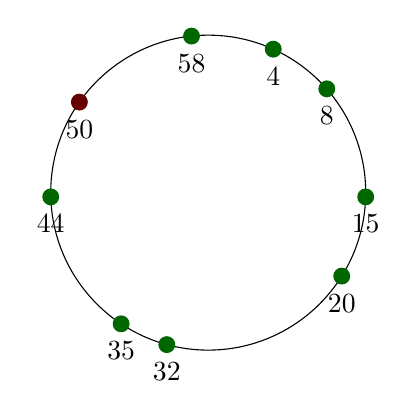
\begin{tikzpicture}[scale=2]
        \draw (0, 0) circle [radius=1];
        \node[draw, fill, circle, inner sep=0,minimum size=2mm,green!40!black, label=below:{$4$}] at (0.413, 0.911){};
        \node[draw, fill, circle, inner sep=0,minimum size=2mm,green!40!black, label=below:{$8$}] at (0.753, 0.659){};
        \node[draw, fill, circle, inner sep=0,minimum size=2mm,green!40!black, label=below:{$15$}] at (1.000, -0.027){};
        \node[draw, fill, circle, inner sep=0,minimum size=2mm,green!40!black, label=below:{$20$}] at (0.848, -0.530){};
        \node[draw, fill, circle, inner sep=0,minimum size=2mm,green!40!black, label=below:{$32$}] at (-0.263, -0.965){};
        \node[draw, fill, circle, inner sep=0,minimum size=2mm,green!40!black, label=below:{$35$}] at (-0.553, -0.833){};
        \node[draw, fill, circle, inner sep=0,minimum size=2mm,green!40!black, label=below:{$44$}] at (-1.000, -0.027){};
        \node[draw, fill, circle, inner sep=0,minimum size=2mm,red!40!black, label=below:{$50$}] at (-0.818, 0.575){};
        \node[draw, fill, circle, inner sep=0,minimum size=2mm,green!40!black, label=below:{$58$}] at (-0.106, 0.994){};
    \end{tikzpicture}
\end{figure}

\section{Transport Layer}
\subsection{Network Applications}
\begin{itemize}[nosep]
    \item Centralized and Peer-to-peer arhictectures
    \item How to design and write network applications
    \item Case studies
          \begin{itemize}[nosep]
              \item HTTP
              \item DNS
              \item P2P applications
          \end{itemize}
    \item These applications need a \emph{reliable method to send information across the network}
    \item Transport Layer provides that service
\end{itemize}
\subsection{Transport Layer}
\begin{itemize}
    \item Transport protocols sit on top of network layer and provide
          \begin{itemize}[nosep]
              \item Application-level multiplexing (``ports'')
              \item Error detection, reliability, etc.
          \end{itemize}
\end{itemize}
\subsection{Error Detection}
\begin{itemize}[nosep]
    \item Idea: add redundant information to catch errors in packet
    \item Three examples
          \begin{itemize}[nosep]
              \item Parity
              \item Internet Checksum
              \item CRC
          \end{itemize}
\end{itemize}
\subsubsection{Parity Bit}
\begin{itemize}[nosep]
    \item Can detect odd number of bit errors
    \item No correction

          \begin{table}[H]
              \begin{tabular}{ll}
                  Data     & 1101101                   \\
                  Parity   & \textcolor{red}{1}        \\
                  Transmit & 1101101\textcolor{red}{1}
              \end{tabular}
          \end{table}
          \url{https://en.wikipedia.org/wiki/Parity_bit}
\end{itemize}

\subsubsection{2-D Parity}
\begin{figure}[H]
    \tikzsetnextfilename{2d-parity}
    \begin{tikzpicture}[node distance=0.1cm]
        \node[draw, rectangle] (top) {0101001};
        \node[below=of top,draw, rectangle] (1) {1101001};
        \node[below=of 1,draw, rectangle] (2) {1011110};
        \node[below=of 2,draw, rectangle] (3) {0001110};
        \node[below=of 3,draw, rectangle] (4) {0110100};
        \node[below=of 4,draw, rectangle] (bottom) {1011111};
        \node[fill=teal!40!white,below=0.4cm of bottom,draw,rectangle] (par) {1111011};

        \node[fill=teal!40!white,right=0cm of top, draw, rectangle] (p1) {1};
        \node[fill=teal!40!white,right=0cm of 1, draw, rectangle] {0};
        \node[fill=teal!40!white,right=0cm of 2, draw, rectangle] {1};
        \node[fill=teal!40!white,right=0cm of 3, draw, rectangle] {1};
        \node[fill=teal!40!white,right=0cm of 4, draw, rectangle] {1};
        \node[fill=teal!40!white,right=0cm of bottom, draw, rectangle] {0};
        \node[fill=teal!40!white,right=0cm of par, draw, rectangle] {0};

        \node[align=left, above=of p1] {Parity\\bits};
        \node[align=left, left=of par] {Parity\\byte};

        \draw[red, thick] (2.center) ellipse (1mm and 2mm);

        \draw[<->] ([xshift=-0.2cm]top.north west) -- ([xshift=-0.2cm]bottom.south west) node[pos=0.5, label=left:{Data}] {};
    \end{tikzpicture}
\end{figure}
\begin{itemize}[nosep]
    \item Add 1 parity bit for each 7 bits
    \item Add 1 parity bit for each bit position across the frame
          \begin{itemize}[nosep]
              \item Can correct single-bit errors
              \item Can detect 2- and 3-bit errors, most 4-bit errors
          \end{itemize}
\end{itemize}

\subsubsection{Checksum}
\begin{itemize}[nosep]
    \item Algorithm
          \begin{itemize}[nosep]
              \item Set \texttt{checksum} field to 0
              \item Sum all 16-bit words, adding any carry bits to the LSB (one's complement sum)
              \item Flip bits to get checksum (one's complement)
          \end{itemize}
    \item Transmit: data + checksum
    \item To check: sum whole packet, including sum, should get \texttt{0xffff}
\end{itemize}
\url{https://tools.ietf.org/html/rfc1071}
\subsubsection{How good is it?}
\begin{itemize}[nosep]
    \item 16 bits is not very long
          \begin{itemize}[nosep]
              \item Probability 1-bit error not detected?
          \end{itemize}
    \item Checksum does catch any 1-bit error
    \item But not any 2-bit error
          \begin{itemize}[nosep]
              \item e.g. increment word ending 0, decrement one ending in 1
          \end{itemize}
\end{itemize}

\subsubsection{CRC -- Error Detection with Polynomials}
\begin{itemize}[nosep]
    \item Consider message to be a polynomial in $\mathbb{Z}_2[x]$
          \begin{itemize}[nosep]
              \item Each bit is one coefficient
              \item e.g. message $10101001 \to m(x) = x^7 + x^5 + x^3 + 1$
          \end{itemize}
    \item Can reduce one polynomial modulo another
          \begin{itemize}[nosep]
              \item Select a degree $k$ \emph{irreducible} polynomial $C(x)$ in $\mathbb{Z}_2[x]$
              \item Let $n(x) = m(x)\cdot x^k$
              \item Compute $r(x) = n(x) \bmod C(x)$
              \item Compute $n(x) - r(x)$
          \end{itemize}
    \item Checking CRC is easy
          \begin{itemize}
              \item Reduce message by $C(x)$, make sure remainder is 0
          \end{itemize}
\end{itemize}
\subsection{Reliable Delivery}
\begin{itemize}
    \item Error detection can discard bad packets
    \item Problem: if bad packets are lost, how can we ensure reliable delivery?
          \begin{itemize}[nosep]
              \item Exactly-once semantics = at least once + at most once
          \end{itemize}
\end{itemize}

\subsubsection{At Least Once Semantics}
\begin{itemize}[nosep]
    \item How can the sender know the packet arrived \emph{at least once}?
          \begin{itemize}[nosep]
              \item Acknowledgements + Timeout
          \end{itemize}
    \item Stop and Wait Protocol
          \begin{itemize}[nosep]
              \item S: Sent packet, wait
              \item R: Receive packet, send ACK
              \item S: Receive ACK, send next packet
              \item S: No ACK, timeout and retransmit
          \end{itemize}
\end{itemize}

\subsubsection{Stop and Wait Problems}
\begin{itemize}[nosep]
    \item Duplicate Data
    \item Duplicate ACKs
    \item Can't fill pipe
    \item Difficult to set the timeout value
\end{itemize}

\subsubsection{At Most Once Semantics}
\begin{itemize}[nosep]
    \item How to avoid duplicates?
          \begin{itemize}[nosep]
              \item Uniquely identify each packet
              \item Have receiver and sender remember
          \end{itemize}
    \item Stop and wait: add 1 bit to the header
          \begin{itemize}[nosep]
              \item Why is it enough?
          \end{itemize}
\end{itemize}

\subsection{Sliding Window Protocol}
\begin{itemize}[nosep]
    \item Still have the problem of keeping pipe full.
          \begin{itemize}[nosep]
              \item Generalize approach > 1-bit counter
              \item Allow multiple outstanding (unACKed) frames
              \item Upper bound on unACKed frames, called \emph{window}
          \end{itemize}
\end{itemize}

\subsubsection{Sliding Window Sender}
\begin{itemize}
    \item Assign sequence number (\texttt{SeqNum}) to each frame
    \item Maintain three state variables
          \begin{itemize}[nosep]
              \item send window size (\texttt{SWS})
              \item last acknowledgement received (\texttt{LAR})
              \item last frame send (\texttt{LFS})
          \end{itemize}
    \item Maintain invariant: $\texttt{LFS} - \texttt{LAR} \leq \texttt{SWS}$
    \item Advance \texttt{LAR} when ACK arrives
    \item Buffer up to \texttt{SWS} frames
\end{itemize}

\subsubsection{Sliding Window Receiver}
\begin{itemize}
    \item Maintain three state variables
          \begin{itemize}[nosep]
              \item receive window size (\texttt{RWS})
              \item largest acceptable frame (\texttt{LAF})
              \item last frame received (\texttt{LFR})
          \end{itemize}
    \item Maintain invariant: $\texttt{LAF} - \texttt{LFR} \leq \texttt{RWS}$
    \item Frame \texttt{SeqNum} arrives:
          \begin{itemize}[nosep]
              \item if $\texttt{LFR} < \texttt{SeqNum} \leq \texttt{LAF}$, accept
              \item if $\texttt{SeqNum} \leq \texttt{LFR}$ or $\texttt{SeqNum} > \texttt{LAF}$, discard
          \end{itemize}
    \item Send \emph{cumulative} ACKs
\end{itemize}